\documentclass{beamer}

\usetheme{egi}

\usepackage[utf8x]{inputenc}
\usepackage[T1]{fontenc}
\usepackage{cmap}
\usepackage{lmodern}
\usepackage[english]{babel}
\usepackage{listings}
\usepackage{color}
\usepackage{url}
\usepackage{hyperref}
\usepackage{verbatim}
\usepackage{fancyvrb,fancybox,calc}
\usepackage{upquote}

% some helpful definitions
\definecolor{opennebulablue}{RGB}{0,145,197}
\definecolor{rubyred}{RGB}{204,52,45}

\newcommand{\opennebul}[1]{Open\textcolor{opennebulablue}{Nebul#1}}
\newcommand{\rocci}{\textcolor{rubyred}{r}\textcolor{opennebulablue}{OCCI}}

\newcommand\Fontsmaller{\fontsize{8}{9.2}\selectfont}
\newcommand\Fonttiny{\fontsize{7}{8.2}\selectfont}

\newcommand{\terminalbox}[2][\Fontsmaller]{
  \begin{Sbox}
  #1
  \begin{minipage}{\linewidth-2\fboxsep-2\fboxrule-4pt}
  \color{white}
  \begin{verbatim}
#2
  \end{verbatim}
  \end{minipage}
  \end{Sbox}
  \fcolorbox{black}{black}{\TheSbox}
}

\lstset{basicstyle=\footnotesize\ttfamily,
  numberstyle=\footnotesize\ttfamily,
  breaklines=true,
  breakatwhitespace=true,
  frame=single,
  numbers=left}


%
\title{Building an OpenNebula Cloud Compliant with EGI FedCloud}
\subtitle{EGI Community Forum 2014}
\author{Boris Par\'ak, CESNET}
\date{2014-05-23, EGI Community Forum 2014, Helsinki}

%\AtBeginPart{\frame{\partpage}}

\begin{document}

\maketitle

\part{Overview}

%%%%%%%%%%%%%%%%%%%%%%%%%%%%%%%%%%%%%%%%%%%%%%%%%%%%%%%%%%%%%%%%%%%%%%%%%%%
\begin{frame}
  \frametitle{Agenda}
  \framesubtitle{}
  \begin{itemize}
    \item OpenNebula in the EGI Federated Cloud
    \item Introduction into OCCI
    \item The rOCCI framework and its components
    \item Hands-on part
      \begin{itemize}
        \item Installation \& configuration of \rocci-server
        \item Installation \& configuration of \rocci-cli
        \item Basic VM life-cycle management tasks
      \end{itemize}
    \item Q \& A
  \end{itemize}
  \hfill
\includegraphics[width=1cm]{images/ruby_logo}
\end{frame}

\part{OCCI}

%%%%%%%%%%%%%%%%%%%%%%%%%%%%%%%%%%%%%%%%%%%%%%%%%%%%%%%%%%%%%%%%%%%%%%%%%%%
\begin{frame}
  \frametitle{OCCI}
  \framesubtitle{What is OCCI?}

  \begin{itemize}
    \item OCCI $\rightarrow$ Open Cloud Computing Interface
    \item OGF standard; Core, Infrastructure and HTTP rendering (GFD.183 - 185)
    \item text-based protocol and API focusing on interoperability in the cloud
    \item designed with IaaS clouds in mind
    \item extensible; used for PaaS, SaaS, Brokering, \dots
  \end{itemize}

  \vspace{0.5cm}
  \hfill 
\includegraphics[width=2.5cm]{images/OCCI_tagline}
\end{frame}

%%%%%%%%%%%%%%%%%%%%%%%%%%%%%%%%%%%%%%%%%%%%%%%%%%%%%%%%%%%%%%%%%%%%%%%%%%%
\begin{frame}
  \frametitle{OCCI}
  \framesubtitle{Core}

  \begin{center}
    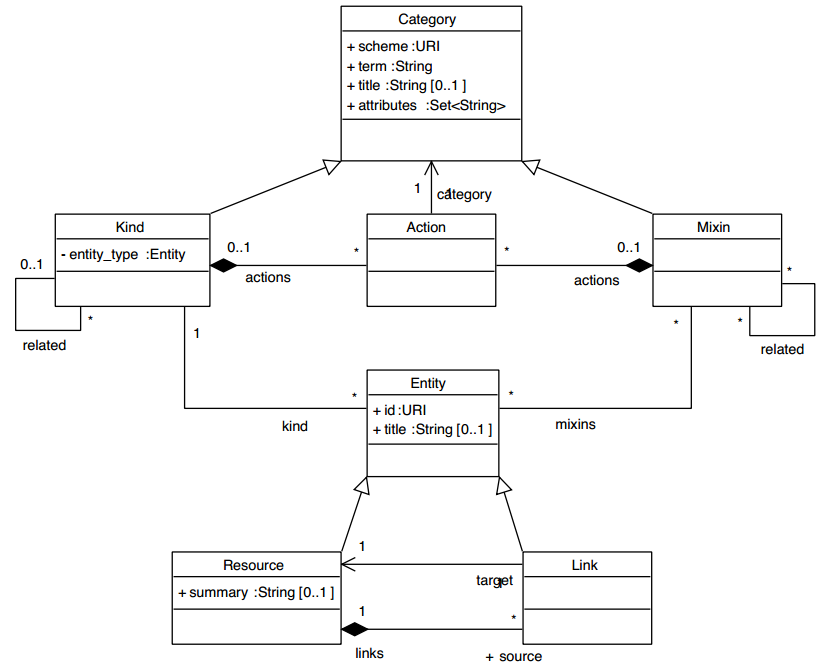
\includegraphics[width=9cm]{images/occi_core_spec}
  \end{center}
\end{frame}

%%%%%%%%%%%%%%%%%%%%%%%%%%%%%%%%%%%%%%%%%%%%%%%%%%%%%%%%%%%%%%%%%%%%%%%%%%%
\begin{frame}
  \frametitle{OCCI}
  \framesubtitle{Infrastructure}

  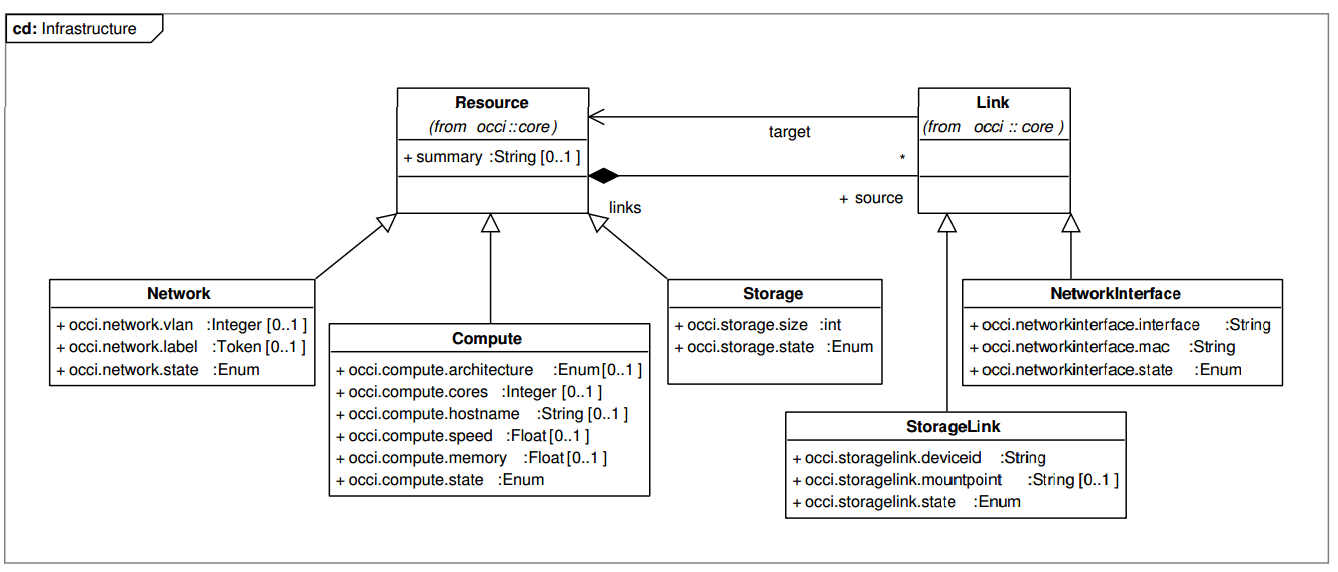
\includegraphics[width=11cm]{images/occi_infra_spec}
\end{frame}

%%%%%%%%%%%%%%%%%%%%%%%%%%%%%%%%%%%%%%%%%%%%%%%%%%%%%%%%%%%%%%%%%%%%%%%%%%%
\begin{frame}
  \frametitle{OCCI}
  \framesubtitle{IaaS Capabilities}

  \begin{columns}
  \begin{column}{0.5\textwidth}
    \begin{enumerate}
        \item Creating VMs
        \item Querying VMs
        \item Destroying VMs
        \item Triggering basic actions on VMs
        \item Creating block storage
        \item Destroying block storage
    \end{enumerate}
  \end{column}

  \begin{column}{0.5\textwidth}
    \begin{enumerate}
    \setcounter{enumi}{6}
        \item Attaching block storage to VMs
        \item Detaching block storage from VMs
        \item Attaching network interfaces to VMs
        \item Detaching network interfaces from VMs
        \item Using contextualization to modify VMs on boot
    \end{enumerate}
  \end{column}
  \end{columns}
\end{frame}

%%%%%%%%%%%%%%%%%%%%%%%%%%%%%%%%%%%%%%%%%%%%%%%%%%%%%%%%%%%%%%%%%%%%%%%%%%%
\begin{frame}[fragile]
  \frametitle{OCCI}
  \framesubtitle{HTTP Rendering}

\begin{terminalbox}{}
POST /compute/ HTTP/1.1

Category: compute;
          scheme="http://.../occi/infrastructure#";
          class="kind"
Category: debian7;
          scheme="http://.../infrastructure/os_tpl#";
          class="mixin"
Category: small;
          scheme="http://.../infrastructure/resource_tpl#";
          class="mixin"
X-OCCI-Attribute: occi.core.title="TestROCCI1"
X-OCCI-Attribute: occi.compute.cores=2
X-OCCI-Attribute: occi.compute.memory=1.7
\end{terminalbox}
\end{frame}

%%%%%%%%%%%%%%%%%%%%%%%%%%%%%%%%%%%%%%%%%%%%%%%%%%%%%%%%%%%%%%%%%%%%%%%%%%%
\begin{frame}
  \frametitle{OCCI}
  \framesubtitle{The rOCCI framework}

  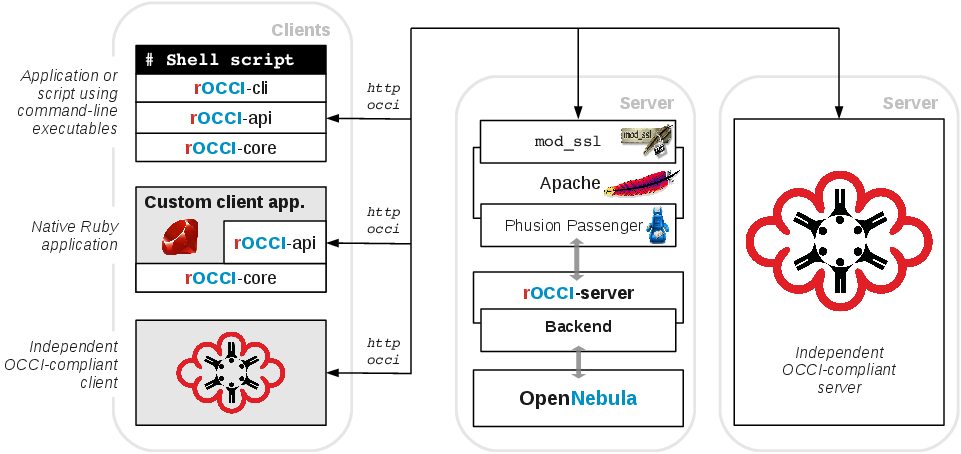
\includegraphics[width=11cm]{images/OCCI_client_servers}
\end{frame}

\part{Before Installation}

%%%%%%%%%%%%%%%%%%%%%%%%%%%%%%%%%%%%%%%%%%%%%%%%%%%%%%%%%%%%%%%%%%%%%%%%%%%
\begin{frame}
  \frametitle{Hands-on}
  \framesubtitle{Beware}

  \begin{center}
    
\includegraphics[width=7cm]{images/warning_logo.png}
  \end{center}
\end{frame}

%%%%%%%%%%%%%%%%%%%%%%%%%%%%%%%%%%%%%%%%%%%%%%%%%%%%%%%%%%%%%%%%%%%%%%%%%%%
\begin{frame}[fragile]
  \frametitle{Before Installation}
  \framesubtitle{Repositories}

\begin{terminalbox}{\Fonttiny}
~# EPEL=http://dl.fedoraproject.org/pub/epel
~# rpm -ivh $EPEL/6/x86_64/epel-release-6-8.noarch.rpm
~# yum install -y gcc-c++ curl-devel httpd \
                  httpd-devel apr-devel apr-util-devel mod_ssl \
                  policycoreutils-python mod_security memcached \
                  openssl-devel zlib-devel git

~# APPDB=http://repository.egi.eu/community/software/rocci.server
~# wget $APPDB/1.0.x/releases/repofiles/sl-6-x86_64.repo \
        -O /etc/yum.repos.d/rocci-server-sl-6-x86_64.repo

~# APPDB=http://repository.egi.eu/community/software/rocci.cli
~# wget $APPDB/4.2.x/releases/repofiles/sl-6-x86_64.repo \
        -O /etc/yum.repos.d/rocci-cli-sl-6-x86_64.repo
\end{terminalbox}
\end{frame}

\part{Sever Installation}

%%%%%%%%%%%%%%%%%%%%%%%%%%%%%%%%%%%%%%%%%%%%%%%%%%%%%%%%%%%%%%%%%%%%%%%%%%%
\begin{frame}[fragile]
  \frametitle{Installation}
  \framesubtitle{rOCCI-server}

  \begin{Sbox}
  \Fonttiny
  \begin{minipage}{\linewidth-2\fboxsep-2\fboxrule-4pt}
  \color{white}
  \begin{verbatim}
~# yum install -y occi-server

~# /opt/occi-server/embedded/bin/passenger-install-apache2-module \
   --auto --languages ruby
~# /opt/occi-server/embedded/bin/passenger-install-apache2-module \
   --snippet > /etc/httpd/conf.d/passenger.conf

~# echo "Listen 11443" >> /etc/httpd/conf/httpd.conf
  \end{verbatim}
  \end{minipage}
  \end{Sbox}
  \fcolorbox{black}{black}{\TheSbox}

  \hfill\\

  \begin{Sbox}
  \Fonttiny
  \begin{minipage}{\linewidth-2\fboxsep-2\fboxrule-4pt}
  \color{white}
  \begin{verbatim}
~# sed -i 's/SELINUX\s*=\s*enforcing/SELINUX=permissive/' \
          /etc/selinux/config
~# setenforce 0
  \end{verbatim}
  \end{minipage}
  \end{Sbox}
  \fcolorbox{black}{black}{\TheSbox}
\end{frame}

%%%%%%%%%%%%%%%%%%%%%%%%%%%%%%%%%%%%%%%%%%%%%%%%%%%%%%%%%%%%%%%%%%%%%%%%%%%
\begin{frame}[fragile]
  \frametitle{Configuration}
  \framesubtitle{rOCCI-server}

  \begin{Sbox}
  \Fontsmaller
  \begin{minipage}{\linewidth-2\fboxsep-2\fboxrule-4pt}
  \color{white}
  \begin{verbatim}
~# su - oneadmin
~$ oneuser create rocci '<actual_password_edited_out>' \
   --driver server_cipher
~$ oneuser chgrp rocci oneadmin
~$ exit
  \end{verbatim}
  \end{minipage}
  \end{Sbox}
  \fcolorbox{black}{black}{\TheSbox}

  \hfill \\

  \begin{Sbox}
  \Fontsmaller
  \begin{minipage}{\linewidth-2\fboxsep-2\fboxrule-4pt}
  \color{white}
  \begin{verbatim}
~# vim /etc/httpd/conf.d/occi-ssl
  \end{verbatim}
  \end{minipage}
  \end{Sbox}
  \fcolorbox{black}{black}{\TheSbox}

  \hfill \\

  \begin{center}
    Remove SSL directives, change protocol to \textbf{http}, authentication\\
    method to \textbf{basic} and the backend to \textbf{opennebula}.
  \end{center}

  \hfill \\

  \begin{Sbox}
  \Fontsmaller
  \begin{minipage}{\linewidth-2\fboxsep-2\fboxrule-4pt}
  \color{white}
  \begin{verbatim}
~# service httpd restart
  \end{verbatim}
  \end{minipage}
  \end{Sbox}
  \fcolorbox{black}{black}{\TheSbox}
\end{frame}

\part{Client Installation}

%%%%%%%%%%%%%%%%%%%%%%%%%%%%%%%%%%%%%%%%%%%%%%%%%%%%%%%%%%%%%%%%%%%%%%%%%%%
\begin{frame}[fragile]
  \frametitle{Installation}
  \framesubtitle{rOCCI-cli}

  \begin{Sbox}
  \Fontsmaller
  \begin{minipage}{\linewidth-2\fboxsep-2\fboxrule-4pt}
  \color{white}
  \begin{verbatim}
~# yum install occi-cli
~# /opt/occi-cli/bin/occi -d -v
~# ln -sf /opt/occi-cli/bin/occi /usr/bin/occi
  \end{verbatim}
  \end{minipage}
  \end{Sbox}
  \fcolorbox{black}{black}{\TheSbox}

  \hfill\\
  \begin{center}
    If you have \textbf{RVM} installed, disable it before running packaged \rocci-cli!
  \end{center}
\end{frame}

\part{Client Usage}

%%%%%%%%%%%%%%%%%%%%%%%%%%%%%%%%%%%%%%%%%%%%%%%%%%%%%%%%%%%%%%%%%%%%%%%%%%%
\begin{frame}[fragile]
  \frametitle{Usage}
  \framesubtitle{rOCCI-cli}

  \begin{Sbox}
  \Fontsmaller
  \begin{minipage}{\linewidth-2\fboxsep-2\fboxrule-4pt}
  \color{white}
  \begin{verbatim}
~# occi --endpoint http://localhost:11443/ --action list \
        --resource os_tpl --auth basic --username onetest-admin \
        --password onetest-admin
~# occi --endpoint http://localhost:11443/ --action list \
        --resource resource_tpl --auth basic --username onetest-admin \
        --password onetest-admin
~# occi --endpoint http://localhost:11443/ --action create \
        --resource compute --mixin os_tpl#uuid_ttylinux_0 \
        --attribute occi.core.title="My rOCCI VM" \
        --auth basic --username onetest-admin \
        --password onetest-admin

~# occi ... --action describe --resource /compute/0 ...
~# occi ... --action delete --resource /compute/0 ...
  \end{verbatim}
  \end{minipage}
  \end{Sbox}
  \fcolorbox{black}{black}{\TheSbox}
\end{frame}

\part{Q \& A}

%%%%%%%%%%%%%%%%%%%%%%%%%%%%%%%%%%%%%%%%%%%%%%%%%%%%%%%%%%%%%%%%%%%%%%%%%%%
\begin{frame}
  \frametitle{References}
  \framesubtitle{OCCI}

  \begin{itemize}
    \item OCCI -- \url{http://occi-wg.org/}
    \item \rocci-cli -- \url{https://github.com/EGI-FCTF/rOCCI-cli}
    \item \rocci-server -- \url{https://github.com/EGI-FCTF/rOCCI-server}
    \item \rocci-cli packages -- \url{https://appdb.egi.eu/store/software/rocci.cli}
    \item \rocci-server packages -- \url{https://appdb.egi.eu/store/software/rocci.server}
  \end{itemize}
\end{frame}

%%%%%%%%%%%%%%%%%%%%%%%%%%%%%%%%%%%%%%%%%%%%%%%%%%%%%%%%%%%%%%%%%%%%%%%%%%%

\begin{frame}
  \frametitle{Q \& A}
  \framesubtitle{}

  \begin{center}
    {\Huge ?}
  \end{center}
\end{frame}


\end{document}
